% !TeX root = ../main.tex
\chapter{Problems and Challenges}
\label{ch:problems}

This chapter provides an honest and comprehensive analysis of the difficulties encountered during the development of the HPC Sorting Serious Game. Understanding these challenges and their solutions is valuable for future developers of educational multiplayer games and contributes to the body of knowledge in serious game development.

%-----------------------------------------------------------------------
\section{Overview}
\label{sec:problems-overview}

Development of a web-first serious game with real-time multiplayer exposed challenges that were tightly coupled: early synchronization faults reduced gameplay trust, UI constraints affected interaction quality, and debugging complexity slowed iteration speed.
% TODO: [Artifact] Case-backed opening mini-narrative (1 concrete failure episode).
% TODO: [Purpose] Ground the chapter in one real incident that links technical failure to educational/usability impact.
% TODO: [Source Inputs] Multiplayer session logs; lobby/startup transition traces; short notes from observed user confusion during affected sessions.
% TODO: [Placement] Immediately after this opening paragraph.
% TODO: [Done Criteria] Include trigger, observed symptom, immediate impact on user understanding/trust, and mitigation pointer.
% TODO: [Cross-refs] Section~\ref{subsec:web-patch-case-study}; Chapter~\ref{ch:results}, Section~\ref{subsec:use-cases}.

The problem space spans multiple domains:

\begin{itemize}
    \item \textbf{Technology selection and framework limitations}: constrained viable implementation paths and introduced replacement/mitigation overhead.
    \item \textbf{Multiplayer state synchronization complexity}: caused divergence risks, ordering issues, and authority conflicts.
    \item \textbf{UI/UX constraints}: touch interaction precision, screen space management, and browser performance variability during collaborative play.
    \item \textbf{Performance optimization requirements}: directly affected playability and perceived responsiveness.
    \item \textbf{Documentation and community support gaps}: increased investigation time and uncertainty in fault attribution.
    \item \textbf{Testing and debugging difficulties}: made timing-dependent defects costly to reproduce and verify.
\end{itemize}

This chapter documents these challenges, the mitigation actions taken, and the resulting lessons that informed subsequent design and evaluation decisions.

%-----------------------------------------------------------------------
\section{Technology Selection Challenges}
\label{sec:technology-challenges}

Selection criteria and the final rationale for tool/framework adoption are presented in Chapter~\ref{ch:methodology} (Section~\ref{sec:technology-selection}). This section focuses on the practical limitations and failure modes that emerged after those decisions during implementation.

%-----------------------------------------------------------------------
\subsection{Game Engine Trade-offs}
\label{subsec:engine-tradeoffs}

% TODO: [Artifact] Concise trade-off comparison table/figure.
% TODO: [Purpose] Connect selection-time assumptions to observed development outcomes.
% TODO: [Source Inputs] Chapter~\ref{ch:methodology}, Section~\ref{subsec:godot-selection}; iteration notes on export stability, plugin readiness, and debugging effort.
% TODO: [Placement] At the end of this subsection, after residual limitations.
% TODO: [Done Criteria] Include at least: iteration speed, export stability, plugin readiness, and debugging effort with one observed impact per criterion.
% TODO: [Cross-refs] Chapter~\ref{ch:methodology}, Section~\ref{sec:technology-selection}.

\textbf{Challenge observed:}
Although Godot remained the best fit overall, development revealed practical constraints in ecosystem maturity and plugin/version compatibility during web-first multiplayer work.

\textbf{Concrete consequence in this project:}
\begin{itemize}
    \item Some networking and editor extensions required additional validation effort before adoption.
    \item Documentation gaps for newer engine paths increased trial-and-error cycles during synchronization debugging.
    \item Export and compatibility checks consumed additional iteration time compared to purely local desktop workflows.
\end{itemize}

\textbf{Mitigation used:}
\begin{itemize}
    \item Scoped architecture boundaries to keep framework/engine-specific code localized.
    \item Used focused prototype loops before integrating new plugin or export assumptions.
    \item Maintained reusable debugging utilities (logging + runtime variable inspection) to shorten diagnosis cycles.
\end{itemize}

\textbf{Residual limitation:}
The solution is robust for current thesis scope, but continued dependency on evolving plugins and browser-export paths remains a maintenance risk for future extensions.

%-----------------------------------------------------------------------
\subsection{GDScript Performance Concerns}
\label{subsec:gdscript-performance}

\textbf{Challenge:} GDScript's interpreted nature raised concerns about performance with 50--200 cards requiring frequent position updates and collision detection.

\textbf{Solution:} Profiling revealed that:
\begin{itemize}
    \item GDScript performance was acceptable for game logic
    \item Bottlenecks were in rendering and physics, handled by Godot's C++ core
    \item Network latency dominated perceived lag, not scripting performance
\end{itemize}

Optimization strategies:
\begin{itemize}
    \item Minimize expensive operations in \texttt{\_process()} and \texttt{\_physics\_process()}
    \item Use object pooling to reduce instantiation overhead
    \item Batch updates where possible
    \item Profile early and often to identify actual bottlenecks
\end{itemize}

%-----------------------------------------------------------------------
\section{GDSync Framework Challenges}
\label{sec:gdsync-challenges}

The most significant technical challenges involved the GDSync framework, which, despite its high-level abstractions, presented several issues.

%-----------------------------------------------------------------------
\subsection{Protected Mode Blocking Issue}
\label{subsec:protected-mode-issue}

\textbf{Challenge:}

GDSync's "protected mode" (default) prevented RPC calls from being executed between non-host peers. When Player A tried to call an RPC on Player B's node, the call would be silently dropped or blocked.

\paragraph*{Error Manifestation:}

\begin{itemize}
    \item Card movement worked from host to clients but not between clients
    \item No error messages or warnings—calls simply failed silently
\end{itemize}

\begin{figure}[htbp]
    \centering
    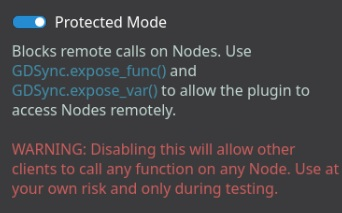
\includegraphics[width=0.6\textwidth]{resources/images/GDSync-protected.png}
    \caption{GDSync's Protected Mode toggle in the plugin settings. When enabled (default), it blocks remote calls on Nodes that haven't been explicitly exposed via \texttt{GDSync.expose\_func()} or \texttt{GDSync.expose\_var()}}
    \label{fig:gdsync-protected}
\end{figure}

\paragraph*{Investigation Process:}

\begin{enumerate}
    \item Verified RPC syntax was correct according to documentation
    \item Added extensive logging to track RPC call flow
    \item Examined GDSync source code to understand permission system
    \item Tested with GDSync's example projects to compare behavior
    \item Posted issue on GDSync GitHub repository
\end{enumerate}

\textbf{Solution:}

\begin{itemize}
    \item Disabled "protected mode" in GDSync configuration
    \item Implemented custom permission checks in application logic
    \item Contributed documentation improvements to GDSync project
    \item Maintained a local fork with a web-export-related framework fix and submitted a pull request to upstream
    \item Shared findings with community to help future users
\end{itemize}

\paragraph*{Lesson Learned:}

% TODO: [Artifact] Traceability evidence block (issue/PR links + short log excerpt figure).
% TODO: [Purpose] Demonstrate how diagnosis decisions were validated and communicated upstream.
% TODO: [Source Inputs] GDSync issue thread, submitted PR, local logger output from failing and fixed runs.
% TODO: [Placement] Immediately below this lesson section.
% TODO: [Done Criteria] Show one evidence item for each step: identification, reproduction, mitigation, and upstream communication.
% TODO: [Cross-refs] Chapter~\ref{ch:implementation}, Section~\ref{subsec:logger-integration}.

The key lessons are tied to specific actions taken in this project:
\begin{itemize}
    \item \textbf{Inspect source, not only docs}: the framework internals were reviewed to verify how protected-mode permissions were enforced; this confirmed that the observed silent RPC drops were policy-driven rather than random transport noise.
    \item \textbf{Isolate failures before full integration}: a minimal multi-instance setup was used to reproduce the same blocked-call pattern across runs; this removed unrelated gameplay complexity from diagnosis.
    \item \textbf{Instrument synchronization paths}: structured logger categories and state tracing were added for call origin, target peer, and outcome; these logs exposed where calls were dropped or reordered.
    \item \textbf{Engage maintainers with actionable evidence}: the issue report included reproducible steps, observed behavior, and mitigation notes, followed by a fork-based patch and PR so thesis progress could continue while upstream review was pending.
\end{itemize}

%-----------------------------------------------------------------------
\subsection{Incomplete Documentation}
\label{subsec:gdsync-documentation}

\textbf{Challenge:}

GDSync documentation covered basic use cases but lacked:
\begin{itemize}
    \item Examples of complex synchronization scenarios
    \item Explanation of internal mechanisms and limitations (These were added during the development of the thesis)
    \item Troubleshooting guides for common problems
    \item Migration guide from vanilla Godot networking
\end{itemize}

\textbf{Impact:}

\begin{itemize}
    \item Trial-and-error approach required for advanced features
    \item Difficulty distinguishing between usage errors and framework bugs
    \item Increased development time
    \item Frustration and consideration of framework replacement
\end{itemize}

\textbf{Mitigation:}

\begin{itemize}
    \item Created internal documentation of discoveries and workarounds
    \item Maintained test project for isolating framework behavior
    \item Contributed examples and documentation improvements to upstream project
    \item Built abstraction layer to isolate GDSync-specific code
\end{itemize}

%-----------------------------------------------------------------------
\subsection{Web Export Signaling Patch Case Study}
\label{subsec:web-patch-case-study}

Web export introduced a mismatch between prototype-era assumptions and browser runtime constraints. During prototyping, GDSync calls were integrated directly; in browser deployment, this path required an interception/replacement layer to keep the original integration style while using a signaling-server-compatible transport flow.


% TODO add links to the relevant issue and PR for this patch in the GDSync repository, along with a short excerpt from the issue discussion and the PR description to show how the problem was identified, mitigated, and communicated to maintainers.
% E.g. the problem with exposing funcitons was that it was not alerting user when using not exposed functions
%  Issue on GDSync repo:
% https://github.com/GD-Sync/GD-Sync/issues/20#issuecomment-3620911143 - [Bug] Multiplayer doesn't work on browser (web export)
% https://github.com/GD-Sync/GD-Sync/issues/107 - [Bug] Web Export Fails with LOCAL_PORT_ERROR - UDP/ENet Not Supported in Browsers  - BY ME
% https://github.com/GD-Sync/GD-Sync/issues/58 - [Help needed] Cannot update remote clients view - BY ME, problem with awaiting frames due to internals of GDSync to instantiate things on other clients
% https://github.com/GD-Sync/GD-Sync/issues/71 - [Help needed] Cannot call functions on remote nodes - BY ME, problem with exposing functions to be called remotely, which is required in protected mode
\textbf{Why this became necessary:}
\begin{itemize}
    \item Browser runtime constraints and export behavior invalidated assumptions from local prototype networking paths.  GDSync uses ENetMultiplayerPeer, which does not work in HTML5 exports at the time of development.
    \item Maintaining thesis velocity favored a compatibility patch over rewriting all synchronization call sites.
    \item The resulting approach replaced/intercepted the local-server path while preserving higher-level game-manager usage of GDSync abstractions.
\end{itemize}

\textbf{Patch components used in this project:}
\begin{itemize}
    \item \texttt{scenes/Multiplayer/GDSyncWebPatch/gdsync\_web\_patch.gd}: applies web-only patch wiring.
    \item \texttt{scenes/Multiplayer/GDSyncWebPatch/local\_server\_signaling.gd}: local-server replacement for signaling/relay mode.
    \item \texttt{scenes/Multiplayer/GDSyncWebPatch/signaling\_client.gd}: HTTP/SSE signaling client behavior.
\end{itemize}

\begin{figure}[htbp]
    \centering
    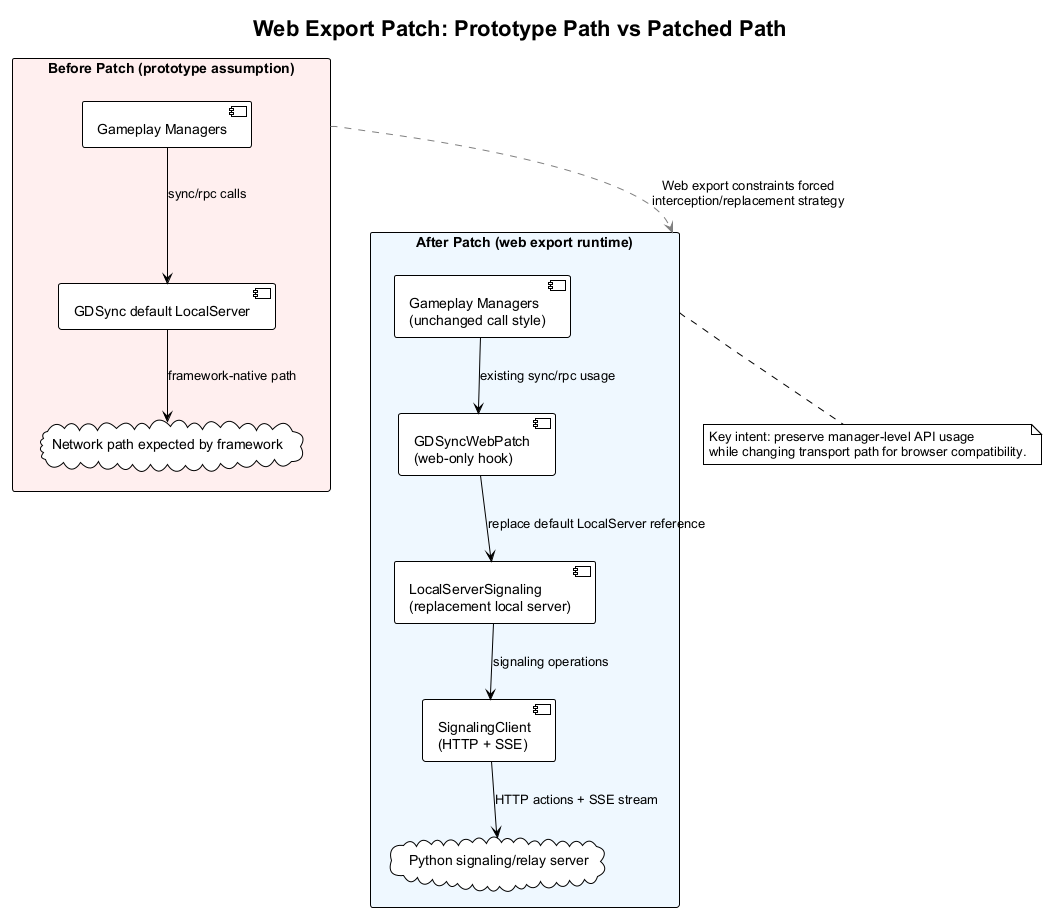
\includegraphics[width=0.95\textwidth]{figures/diagrams/web-patch-before-after}
    \caption{Prototype-to-web architecture diff showing LocalServer interception and relay-based replacement}
    \label{fig:web-patch-before-after}
\end{figure}

\begin{figure}[htbp]
    \centering
    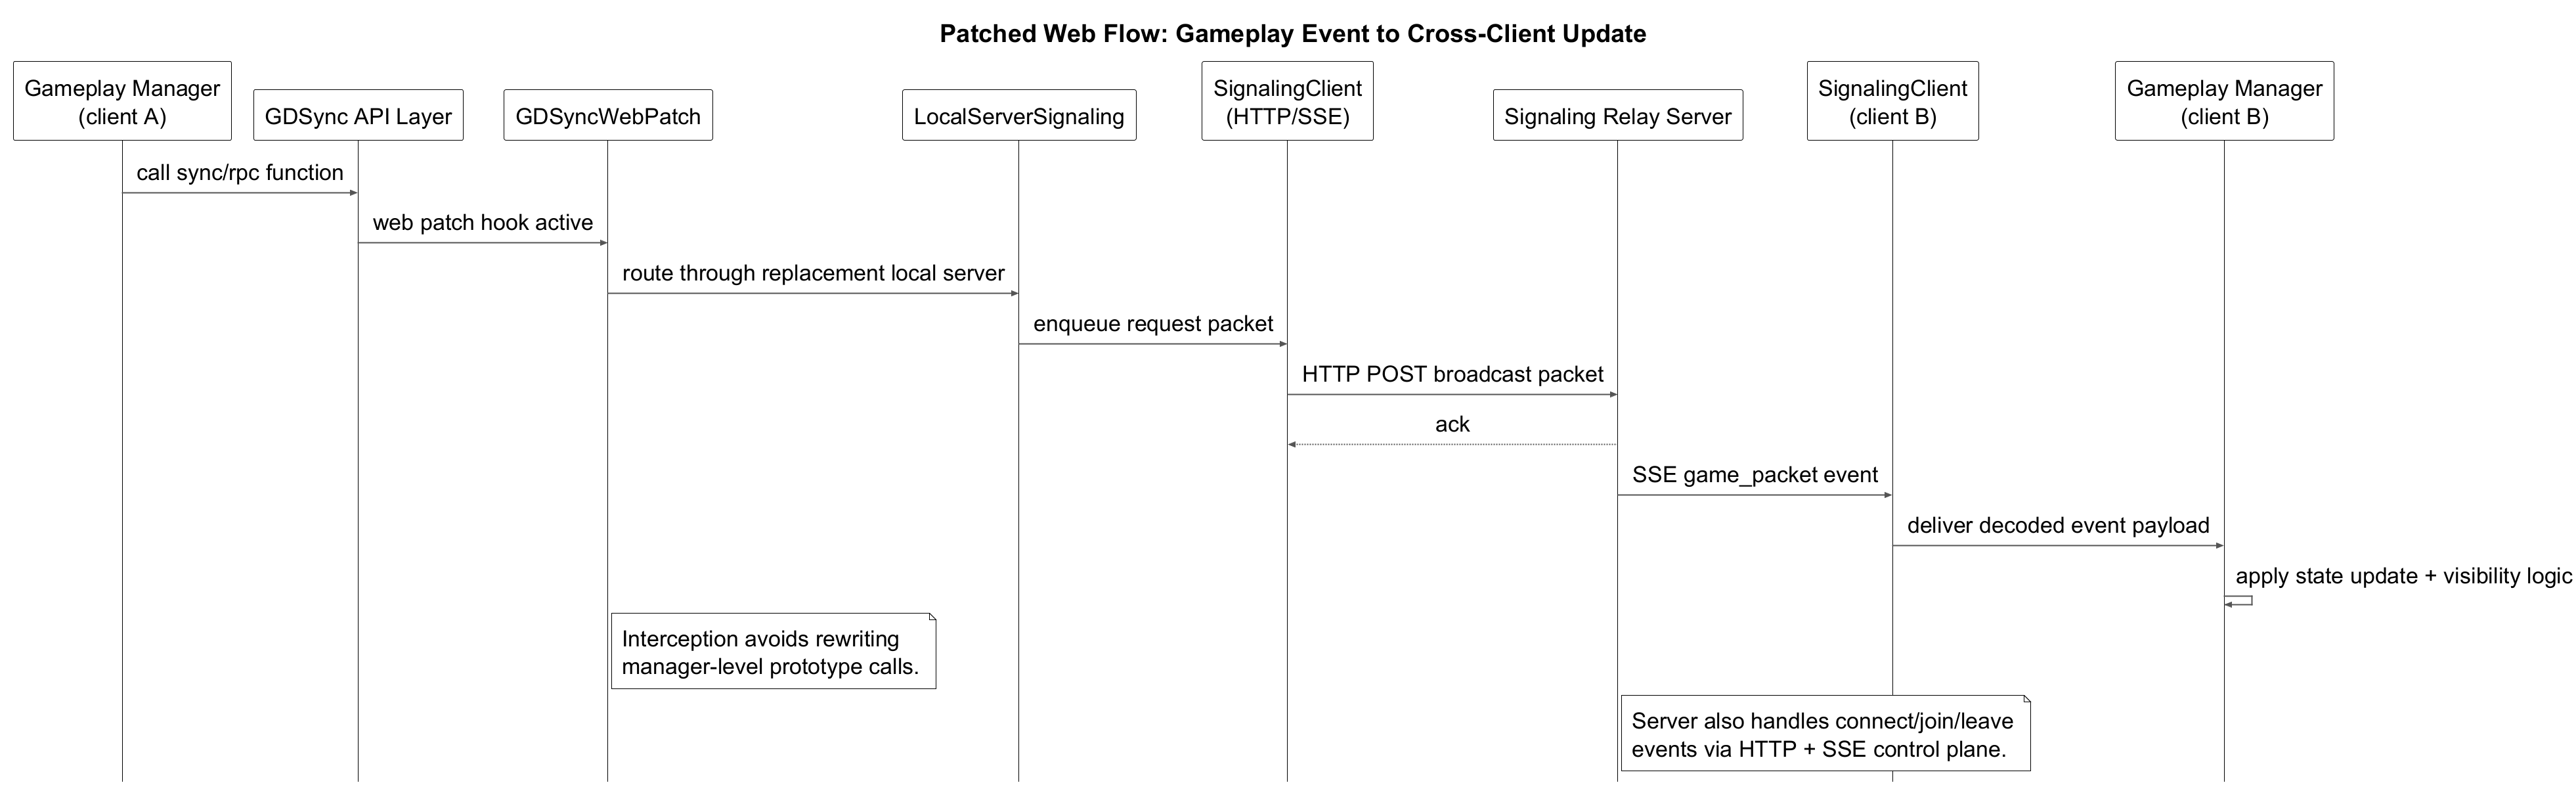
\includegraphics[width=0.95\textwidth]{figures/diagrams/web-patch-packet-event-sequence}
    \caption{Patched web signaling event sequence from gameplay call intent to synchronized client update}
    \label{fig:web-patch-packet-event-sequence}
\end{figure}

\begin{figure}[htbp]
    \centering
    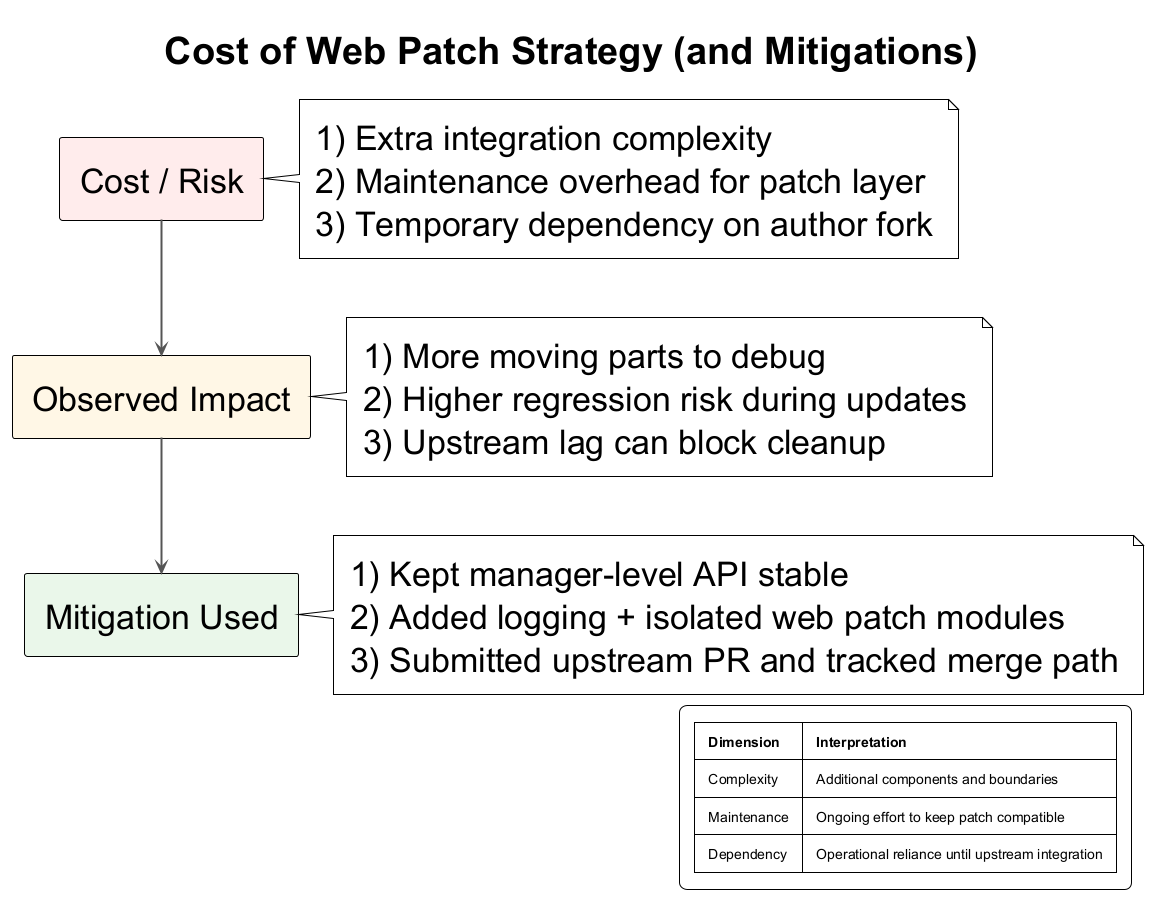
\includegraphics[width=0.9\textwidth]{figures/diagrams/web-patch-cost-summary}
    \caption{Cost of web-patch strategy: added complexity, maintenance burden, and temporary fork dependency}
    \label{fig:web-patch-cost-summary}
\end{figure}

The patch enabled continuity of the existing gameplay integration model but increased maintenance overhead, which is why a fork-plus-PR strategy was used as an interim operational path.

%-----------------------------------------------------------------------
\subsection{Debugging Multiplayer Issues}
\label{subsec:multiplayer-debugging}

\textbf{Challenge:}

Debugging multiplayer code is inherently difficult:
\begin{itemize}
    \item Requires multiple devices or instances
    \item Race conditions and timing-dependent bugs
    \item Network variability complicates reproduction
    \item Limited visibility into remote client state
\end{itemize}

\paragraph*{Solutions Implemented:}

\begin{enumerate}
    \item \textbf{Multi-Instance Testing}: Launched multiple Godot editor instances on the same machine
    \item \textbf{Network Logging}: Comprehensive logging of all network events with timestamps
    \item \textbf{State Dumps}: Ability to print full game state on command
    \item \textbf{Visual Indicators}: On-screen display of connection status, peer IDs, sync status
    \item \textbf{Replay System}: Recorded game events for post-mortem analysis
\end{enumerate}

%-----------------------------------------------------------------------
\section{Multiplayer Synchronization Challenges}
\label{sec:sync-challenges}

%-----------------------------------------------------------------------
\subsection{Card Order Synchronization}
\label{subsec:card-order-sync}

\textbf{Challenge:}

Maintaining consistent card ordering across clients proved more complex than anticipated. Issues included:
\begin{itemize}
    \item Godot's scene tree ordering not guaranteed to match logical ordering
    \item Child node order not automatically synchronized
    \item Timing differences causing transient inconsistencies
\end{itemize}

\textbf{Symptom:}

Cards appeared in different orders on different clients' screens, even though the underlying data was correct.

\textbf{Solution:}

\begin{enumerate}
    \item Implemented explicit position indices for cards
    \item Synchronized card order separately from card positions
    \item Used z-index to control visual stacking order
    \item Periodic consistency checks and resynchronization
\end{enumerate}

\begin{lstlisting}[caption={Card order synchronization approach}]
# Each card has an explicit order index
var card_order_index: int

# Synchronize order explicitly
@GDSync.rpc(call_local=true)
func sync_card_order(card_id: int, new_index: int):
    var card = get_card_by_id(card_id)
    card.card_order_index = new_index
    resort_cards_by_index()
\end{lstlisting}

%-----------------------------------------------------------------------
\subsection{Timing and Race Conditions}
\label{subsec:timing-issues}

\textbf{Challenge:}

Multiplayer systems are susceptible to race conditions:
\begin{itemize}
    \item Simultaneous card movements by different players
    \item Network messages arriving out of order
    \item Inconsistent state when players join mid-game
\end{itemize}

\textbf{Examples:}

\begin{itemize}
    \item Two players drag the same card simultaneously
    \item Player joins lobby after game has started
    \item Card deleted on host but still referenced on client
\end{itemize}

\textbf{Solutions:}

\begin{itemize}
    \item \textbf{Host Authority}: Only host can finalize state changes
    \item \textbf{Client Prediction with Rollback}: Show immediate feedback, then correct if host disagrees
    \item \textbf{State Snapshots}: New players receive full state snapshot on join
    \item \textbf{Defensive Programming}: Check object existence before operations
\end{itemize}

%-----------------------------------------------------------------------
\subsection{Different Client Views}
\label{subsec:client-views}

\textbf{Challenge:}

In multiplayer mode (OpenMP simulation), different players should see different cards in local buffers (simulating thread-private data), but maintaining this selective visibility while synchronizing the shared container was complex.

\paragraph*{Technical Issue:}

GDSync's node replication tries to keep all clients' scene trees identical, but selective visibility required different scene trees per client.

\textbf{Solution:}

\begin{itemize}
    \item Replicate all cards to all clients (for consistency)
    \item Use visibility flags to hide inappropriate cards
    \item Implement client-side filtering based on ownership metadata
    \item Synchronize ownership and visibility separately from positions
\end{itemize}

%-----------------------------------------------------------------------
\section{UI/UX Challenges}
\label{sec:mobile-ux-challenges}

%-----------------------------------------------------------------------
\subsection{Displaying Many Cards on Limited Screen Space}
\label{subsec:many-cards-small-screens}

\textbf{Challenge:}

Displaying 50--200 cards on screen (particularly on smaller browser viewports or touch-enabled devices) presents significant layout challenges:
\begin{itemize}
    \item Cards must be large enough to read and tap
    \item All cards must be accessible without excessive scrolling
    \item Layout must work in both portrait and landscape orientations
\end{itemize}

\paragraph*{Solutions Attempted:}

\begin{enumerate}
    \item \textbf{Grid Layout}: Cards arranged in a grid
          \begin{itemize}
              \item Pros: Space-efficient, familiar pattern
              \item Cons: Hard to see linear order, scrolling still required
          \end{itemize}

    \item \textbf{Scrollable Row (Selected Direction)}: Single row with horizontal scrolling
          \begin{itemize}
              \item Pros: Linear order visible, simple interaction
              \item Cons: Requires substantial scrolling with many cards
          \end{itemize}

    \item \textbf{Zoomable Canvas}: Pan and zoom to navigate cards
          \begin{itemize}
              \item Pros: Flexible navigation, can fit many cards
              \item Cons: Complex interaction, easy to get lost
          \end{itemize}

    \item \textbf{Hybrid Approach (Selected Direction)}:
          \begin{itemize}
              \item Grid layout with intelligent sizing
              \item Vertical scrolling for overflow
              \item Zoom controls for adjusting card size were explored but not fully implemented in the current version
          \end{itemize}
\end{enumerate}

%-----------------------------------------------------------------------
\subsection{Touch Interaction Precision}
\label{subsec:touch-precision}

\textbf{Challenge:}

Touch input is less precise than mouse input:
\begin{itemize}
    \item Finger occludes card being dragged
    \item Difficulty selecting specific cards when densely packed
    \item Accidental touches and swipes
\end{itemize}

\textbf{Solutions:}

\begin{itemize}
    \item \textbf{Offset Dragging}: Card rendered above finger with offset
    \item \textbf{Magnification}: Enlarge selected card for better visibility
    \item \textbf{Touch Feedback}: Visual and haptic feedback for touch events
    \item \textbf{Double-Tap Select}: Alternative to drag for card selection
    \item \textbf{Drop Zone Highlighting}: Clear indication of valid drop targets
\end{itemize}

%-----------------------------------------------------------------------
\subsection{Performance on Low-End Devices}
\label{subsec:lowend-performance}

\textbf{Challenge:}

Not all students have high-end hardware. The game needed to run acceptably across a range of devices and browsers, including low-end laptops and older browser versions.

\paragraph*{Performance Constraints:}

\begin{itemize}
    \item Limited GPU power for rendering many cards
    \item Lower memory (2--4 GB RAM)
    \item Slower network hardware
    \item Battery life concerns
\end{itemize}

\paragraph*{Optimization Strategies Considered:}

The following strategies were evaluated; not all were fully implemented in the current version:
\begin{itemize}
    \item Reduce draw calls through Godot's built-in 2D batching
    \item Viewport culling to avoid rendering off-screen cards (handled by Godot's built-in culling)
    \item Texture atlases to reduce texture swaps when rendering many card sprites
    \item Server-side gzip/Brotli compression of the exported WebAssembly and resource files, reducing the network transfer size from approximately 135~MB to 60~MB
\end{itemize}

Profiling showed that rendering bottlenecks were manageable for the target card counts (1--200), so more aggressive optimizations were not required (see Chapter~\ref{ch:results}, Section~\ref{subsec:export-size}).

%-----------------------------------------------------------------------
\section{Testing Challenges}
\label{sec:testing-challenges}

%-----------------------------------------------------------------------
\subsection{Multiplayer Testing Complexity}
\label{subsec:multiplayer-testing}

\textbf{Challenge:}

Testing multiplayer functionality requires:
\begin{itemize}
    \item Multiple devices or instances
    \item Coordination between test clients
    \item Reproduction of specific network conditions
    \item Testing edge cases (disconnections, late joins, etc.)
\end{itemize}

\paragraph*{Approaches:}

\begin{enumerate}
    \item \textbf{Multi-Instance Browser Testing}: Run multiple browser tabs or windows on development machine
    \item \textbf{Cross-Browser Testing}: Test on Chrome, Firefox, and Edge
    \item \textbf{Automated Test Scenarios}: Scripts to simulate player actions
    \item \textbf{Network Simulation}: Tools to introduce latency and packet loss
\end{enumerate}

\paragraph*{Limitations:}

\begin{itemize}
    \item Automated testing limited for interactive gameplay
    \item Difficult to reproduce exact timing of race conditions
    \item Real-world network conditions vary widely
\end{itemize}

%-----------------------------------------------------------------------
\subsection{Lack of Automated Testing}
\label{subsec:automated-testing}

\textbf{Challenge:}

Godot's testing ecosystem is less mature than traditional software development frameworks:
\begin{itemize}
    \item No built-in unit testing framework
    \item GUI testing particularly difficult
    \item Networking code hard to test in isolation
\end{itemize}

\paragraph*{Approach Taken:}

\begin{itemize}
    \item Manual testing with documented test cases
    \item Integration tests for critical paths
    \item Regression testing checklist before releases
    \item Community feedback as informal usability testing
\end{itemize}

\paragraph*{Future Improvement:}

\begin{itemize}
    \item Integrate GUT (Godot Unit Test) framework
    \item Develop automated test suite for core logic
    \item Implement continuous integration pipeline
\end{itemize}

%-----------------------------------------------------------------------
\section{Educational Design Challenges}
\label{sec:educational-challenges}

%-----------------------------------------------------------------------
\subsection{Balancing Accuracy and Playability}
\label{subsec:accuracy-vs-playability}

\textbf{Challenge:}

Educational games must balance pedagogical accuracy with engaging gameplay. Too much realism can reduce fun; too much simplification can create misconceptions.

\paragraph*{Trade-offs Made:}

\begin{itemize}
    \item \textbf{Simplified Memory Model}: Actual shared-memory systems have complex cache hierarchies not represented
    \item \textbf{Abstracted Synchronization}: Real OpenMP requires explicit barriers, locks, and atomic operations
    \item \textbf{Idealized Performance}: Network latency doesn't perfectly model memory access patterns
\end{itemize}

\textbf{Mitigation:}

\begin{itemize}
    \item Clear framing: "This is a metaphor, not a simulation"
    \item Post-game discussions to connect game to real concepts
    \item Accompanying documentation explaining simplifications
    \item Progressive difficulty introducing more complexity
\end{itemize}

%-----------------------------------------------------------------------
\subsection{Assessment of Learning Effectiveness}
\label{subsec:learning-assessment}

\textbf{Challenge:}

Demonstrating that the game actually improves learning outcomes requires formal educational research, including:
\begin{itemize}
    \item Pre/post-test measurements
    \item Control groups using traditional instruction
    \item Statistical analysis of results
    \item Long-term retention studies
\end{itemize}

\paragraph*{Limitations:}

Within the scope of this thesis, full educational efficacy studies were not feasible due to:
\begin{itemize}
    \item Time constraints
    \item Need for institutional review board approval
    \item Difficulty recruiting sufficient participants
    \item Complexity of isolating game's effect from other factors
\end{itemize}

\paragraph*{Future Work:}

Formal educational evaluation remains an important direction for future research, as discussed in Chapter~\ref{ch:conclusion}.

%-----------------------------------------------------------------------
\section{Lessons Learned}
\label{sec:lessons-learned}

%-----------------------------------------------------------------------
\subsection{Technical Lessons}
\label{subsec:technical-lessons}

\begin{enumerate}
    \item \textbf{Framework Evaluation}: Thoroughly evaluate third-party frameworks before committing; test advanced use cases early.

    \item \textbf{Abstraction Layers}: Isolate framework-specific code to facilitate future replacement if needed.

    \item \textbf{State Management}: Design clear state management patterns early; retrofitting is expensive.

    \item \textbf{Logging Infrastructure}: Comprehensive logging is essential for multiplayer debugging.

    \item \textbf{Performance Profiling}: Profile early and often; don't assume where bottlenecks are.
\end{enumerate}

%-----------------------------------------------------------------------
\subsection{Design Lessons}
\label{subsec:design-lessons}

\begin{enumerate}
    \item \textbf{User Testing}: Conduct user testing early; designer assumptions often wrong.

    \item \textbf{Responsive Design}: Design for varying viewport sizes and input methods from the start, not as an afterthought.

    \item \textbf{Simplicity}: Simpler interactions work better across input methods; complexity reduces usability.

    \item \textbf{Feedback}: Clear, immediate feedback is critical for learning and engagement.
\end{enumerate}

%-----------------------------------------------------------------------
\subsection{Process Lessons}
\label{subsec:process-lessons}

\begin{enumerate}
    \item \textbf{Iterative Development}: Iterative, incremental development surfaced issues early.

    \item \textbf{Version Control}: Frequent commits with clear messages saved time during debugging.

    \item \textbf{Documentation}: Documenting problems and solutions as they occurred proved invaluable.

    \item \textbf{Community Engagement}: Engaging with open-source communities provided solutions and support.
\end{enumerate}

%-----------------------------------------------------------------------
\section{Summary}
\label{sec:problems-summary}

This chapter documented the significant challenges encountered during development:

\begin{itemize}
    \item \textbf{Technology Challenges}: Engine trade-offs, framework limitations, and performance concerns
    \item \textbf{GDSync Issues}: Protected mode blocking, incomplete documentation, and debugging difficulty
    \item \textbf{Synchronization Complexity}: Card ordering, race conditions, and selective visibility
    \item \textbf{UI/UX}: Screen space constraints, touch/mouse interaction precision, and device performance variability
    \item \textbf{Testing Difficulty}: Multiplayer testing complexity and lack of automated testing tools
    \item \textbf{Educational Design}: Balancing accuracy with playability and assessing learning effectiveness
\end{itemize}

Importantly, this chapter also presented solutions and lessons learned that will benefit future developers of similar educational multiplayer games. The next chapter concludes the thesis and discusses future directions for research and development.

